%%%%%%%%%%%%%%%%%%%%%%%%%%%%%%%%%%%%%%%%%%%%%%%%%%%%%%%%%%%%%%%%%%%%%%%%%%%%%%%%%%
\begin{frame}[fragile]\frametitle{}
\begin{center}
{\Large Conclusions}
\end{center}
\end{frame}

%%%%%%%%%%%%%%%%%%%%%%%%%%%%%%%%%%%%%%%%%%%%%%%%%%%%%%%%%%%
\begin{frame}[fragile]\frametitle{Benefits}
      % \begin{center}
        % 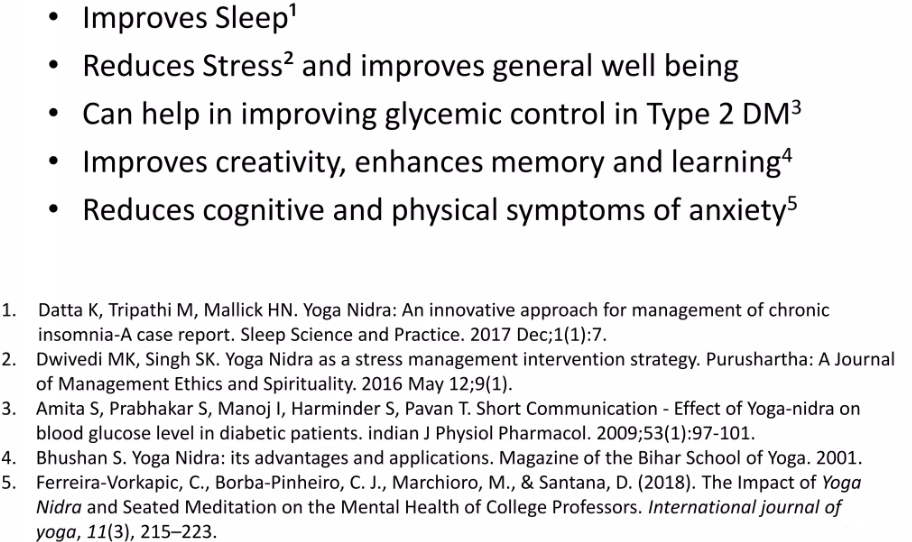
\includegraphics[width=\linewidth,keepaspectratio]{yoganidra11}

        % \end{center}

    \begin{itemize}
        \item Improves Sleep\textsuperscript{1}
        \item Reduces Stress\textsuperscript{2} and improves general well-being
        \item Can help in improving glycemic control in Type 2 DM\textsuperscript{3}
        \item Improves creativity, enhances memory and learning\textsuperscript{4}
        \item Reduces cognitive and physical symptoms of anxiety\textsuperscript{5}
    \end{itemize}
    \begin{itemize}
        \item[1.] Datta K, Tripathi M, Mallick HN. Yoga Nidra: An innovative approach for management of chronic insomnia-A case report. Sleep Science and Practice. 2017 Dec;1(1):7.
        \item[2.] Dwivedi MK, Singh SK. Yoga Nidra as a stress management intervention strategy. Purushartha: A Journal of Management Ethics and Spirituality. 2016 May 12;9(1).
        \item[3.] Amita S, Prabhakar S, Manoj I, Harminder S, Pavan T. Short Communication - Effect of Yoga-nidra on blood glucose level in diabetic patients. Indian J Physiol Pharmacol. 2009;53(1):97-101.
        \item[4.] Bhushan S. Yoga Nidra: its advantages and applications. Magazine of the Bihar School of Yoga. 2001.
        \item[5.] Ferreira-Vorkapic, C., Borba-Pinheiro, C. J., Marchioro, M., \& Santana, D. (2018). The Impact of Yoga Nidra and Seated Meditation on the Mental Health of College Professors. International journal of yoga, 11(3), 215–223.
    \end{itemize}
	
		{\tiny (Ref: Yoga Nidra - Dr Amit Chail)}		

\end{frame}

%%%%%%%%%%%%%%%%%%%%%%%%%%%%%%%%%%%%%%%%%%%%%%%%%%%%%%%%%%%
\begin{frame}[fragile]\frametitle{As behavioral change}
      % \begin{center}
        % 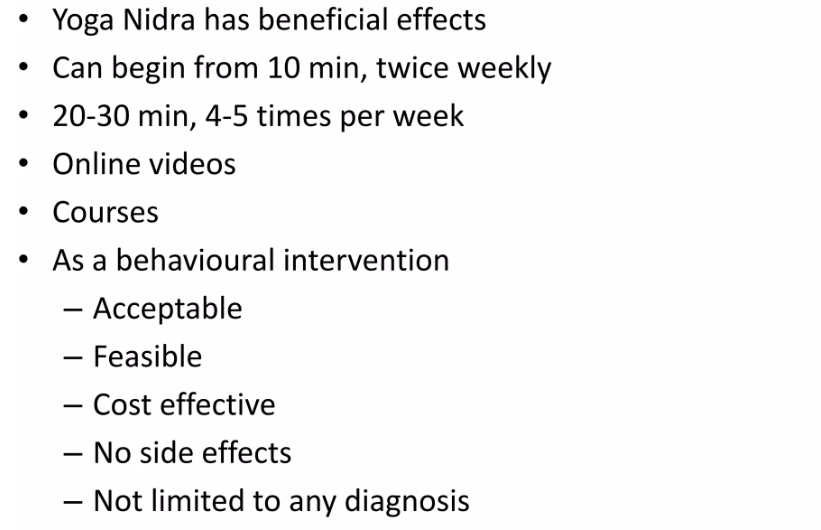
\includegraphics[width=\linewidth,keepaspectratio]{yoganidra12}

        % \end{center}

    \begin{itemize}
        \item Can begin from 10 min, twice weekly, to 20-30 min, 4-5 times per week.
		\item Its is Acceptable, Feasible, Cost Effective, No side effects and can be done while in any diagnosis.
		\item Teaching or coaching can be done in-person or remote, singular or in group, local or global
    \end{itemize}
	
		{\tiny (Ref: Yoga Nidra - Dr Amit Chail)}		

\end{frame}

%%%%%%%%%%%%%%%%%%%%%%%%%%%%%%%%%%%%%%%%%%%%%%%%%%%%%%%%%%%
\begin{frame}[fragile]\frametitle{Additional Benefits}
    \begin{itemize}
        \item \textbf{Mental Benefits:}
        \begin{itemize}
            \item Increased learning capabilities
            \item Enhanced memory and intuition
            \item Boosted creativity
            \item Mental reprogramming capabilities
        \end{itemize}
        \item \textbf{Physiological Benefits:}
        \begin{itemize}
            \item Balanced nervous system
            \item Increased endorphin production
            \item Reduced cortisol and noradrenaline levels
            \item Deep skeletal-muscular relaxation
        \end{itemize}
        \item \textbf{Therapeutic Applications:}
        \begin{itemize}
            \item Relief from depression and anxiety
            \item Help with insomnia and headaches
            \item Management of fibromyalgia
            \item Treatment of chronic fatigue
            \item Support for hypertension
        \end{itemize}
    \end{itemize}
\end{frame}

%%%%%%%%%%%%%%%%%%%%%%%%%%%%%%%%%%%%%%%%%%%%%%%%%%%%%%%%%%%
\begin{frame}[fragile]\frametitle{Summary}
      % \begin{center}
        % 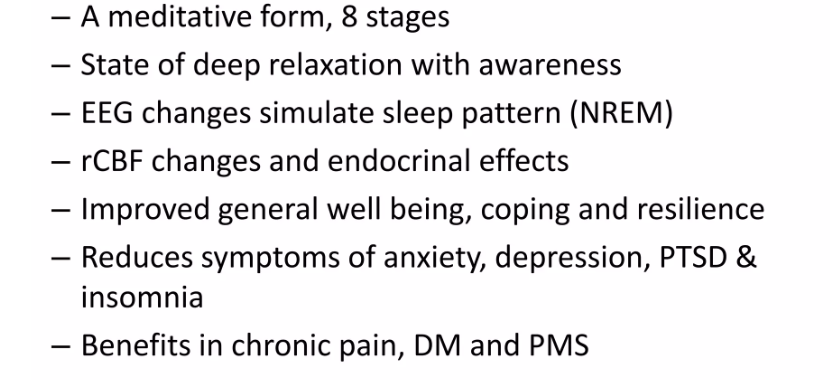
\includegraphics[width=\linewidth,keepaspectratio]{yoganidra13}

        % \end{center}

    \begin{itemize}
        \item A meditative form, 8 stages
        \item State of deep relaxation with awareness
        \item EEG changes simulate sleep pattern (NREM)
        \item rCBF changes and endocrinal effects
        \item Improved general well-being, coping, and resilience
        \item Reduces symptoms of anxiety, depression, PTSD \& insomnia
        \item Benefits in chronic pain, DM, and PMS
    \end{itemize}
	
		{\tiny (Ref: Yoga Nidra - Dr Amit Chail)}		

\end{frame}

%%%%%%%%%%%%%%%%%%%%%%%%%%%%%%%%%%%%%%%%%%%%%%%%%%%%%%%%%%%%%%%%%%%%%%%%%%%%%%%%%%
\begin{frame}[fragile]\frametitle{Integrating Into Daily Life}
    \begin{itemize}
        \item \textbf{Morning Practice:}
        \begin{itemize}
            \item Sets positive tone for day
            \item Enhances mental clarity
            \item Boosts energy levels
        \end{itemize}
        \item \textbf{Midday Reset:}
        \begin{itemize}
            \item Reduces workplace stress
            \item Improves focus and productivity
            \item Quick restoration (15-20 minutes)
        \end{itemize}
        \item \textbf{Evening Practice:}
        \begin{itemize}
            \item Prepares for restful sleep
            \item Releases daily tension
            \item Processes emotional residue
        \end{itemize}
    \end{itemize}
\end{frame}

%%%%%%%%%%%%%%%%%%%%%%%%%%%%%%%%%%%%%%%%%%%%%%%%%%%%%%%%%%%%%%%%%%%%%%%%%%%%%%%%%%
\begin{frame}[fragile]\frametitle{Common Challenges and Solutions}
    \begin{itemize}
        \item \textbf{Falling Asleep:}
        \begin{itemize}
            \item Practice at times of higher energy
            \item Maintain lighter room temperature
            \item Keep eyes slightly open
        \end{itemize}
        \item \textbf{Racing Thoughts:}
        \begin{itemize}
            \item Focus more on physical sensations
            \item Return to breath awareness
            \item Practice regularly to improve focus
        \end{itemize}
        \item \textbf{Physical Discomfort:}
        \begin{itemize}
            \item Use additional props as needed
            \item Adjust position before starting
            \item Practice progressive muscle relaxation
        \end{itemize}
    \end{itemize}
\end{frame}

%%%%%%%%%%%%%%%%%%%%%%%%%%%%%%%%%%%%%%%%%%%%%%%%%%%%%%%%%%%%%%%%%%%%%%%%%%%%%%%%%%
\begin{frame}[fragile]\frametitle{Resources for Further Reading}
    \begin{itemize}
        \item \textbf{Books:}
        \begin{itemize}
            \item "Yoga Nidra" by Swami Satyananda Saraswati.
            \item "Yoga Nidra: A Meditative Practice for Deep Relaxation and Healing" by Richard Miller.
            \item "Yoga Nidra: The Art of Transformational Sleep" by Kamini Desai.
        \end{itemize}
		\item ``Yoga Nidra Script - 8 Stage for Anxiety \& Stress Management (40 mins practice)'' https://www.tummee.com/yoga-philosophy/yoga-nidra-script-anxiety-8-stage-40-mins
    \end{itemize}
\end{frame}